\documentclass[dvipsnames,png,border=10pt,tikz]{standalone}
\usepackage{tikz}
\usetikzlibrary{shapes.geometric} % required for the ellipse shape
\usetikzlibrary{arrows, backgrounds, calc, positioning}

\tikzset{vertex style/.style={
    draw=#1,
    thick,
    fill=#1!70,
    text=white,
    ellipse,
    minimum width=1cm,
    minimum height=1cm,
    font=\small,
    outer sep=3pt,
  },
	text style/.style={
    sloped, % the text will be parallel to the connection 
    text=black,
    font=\footnotesize,
    above
  }
}
\begin{document}
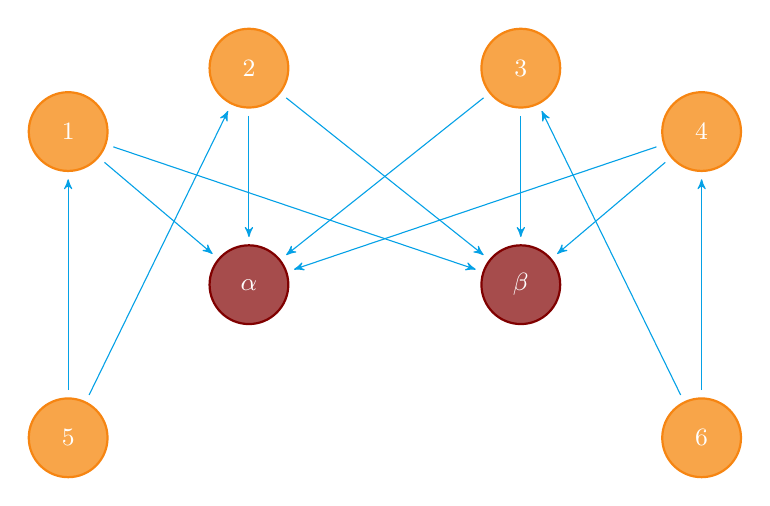
\begin{tikzpicture}[node distance=2.75cm,>=stealth']
%\node[vertex style=Turquoise] (KB) {Knowledge Base};

\node[vertex style=Maroon, xshift=-2em] (nodeA) {\begin{math}\alpha \end{math}};
\node[vertex style=Maroon, right of=nodeA, xshift=2em] (nodeB) {\begin{math}\beta \end{math}};

\node[vertex style=BurntOrange, above left of=nodeA,xshift=-1em] (node1) {1}
 edge [->,cyan!90!blue] node[text style,above]{} (nodeA)
 edge [->,cyan!90!blue] node[text style,above]{} (nodeB);

\node[vertex style=BurntOrange, above of=nodeA] (node2) {2}
 edge [->,cyan!90!blue] node[text style,above]{} (nodeA)
 edge [->,cyan!90!blue] node[text style,above]{} (nodeB);

\node[vertex style=BurntOrange, above of=nodeB] (node3) {3}
 edge [->,cyan!90!blue] node[text style,above]{} (nodeA)
 edge [->,cyan!90!blue] node[text style,above]{} (nodeB);

\node[vertex style=BurntOrange, above right of=nodeB,xshift=1em] (node4) {4}
 edge [->,cyan!90!blue] node[text style,above]{} (nodeA)
 edge [->,cyan!90!blue] node[text style,above]{} (nodeB);


\node[vertex style=BurntOrange, below left of=nodeA,xshift=-1em] (node5) {5}
%\node[vertex style=BurntOrange, above of=node1,xshift=1em] (node5) {5}
 edge [->,cyan!90!blue] node[text style,above]{} (node1)
 edge [->,cyan!90!blue] node[text style,above]{} (node2);

\node[vertex style=BurntOrange, below right of=nodeB,xshift=1em] (node6) {6}
%\node[vertex style=BurntOrange, above of=node2,xshift=5em] (node6) {6}
 edge [->,cyan!90!blue] node[text style,above]{} (node3)
 edge [->,cyan!90!blue] node[text style,above]{} (node4);


\end{tikzpicture}

\end{document}
